\section{Adaptive Komponente in Hadoop}
\label{sec:inriaSetting}

\todo{Text besser an neue unterabschnitte anpassen}
Eine normale Hadoop"=Installation besitzt keine adaptive Komponente, sondern rein statische Einstellungen.
Um damit Hadoop zu optimieren, müssen die Einstellungen immer manuell auf den jeweils benötigten Anwendungstyp angepasst werden.
Dazu gibt es auch bereits verschiedene Scheduler, den \emph{Fair Scheduler}, welcher alle Anwendungen ausführt und ihnen gleich viele Ressourcen zuteilt, und den \emph{Capacity Scheduler}.
Letzterer sorgt dafür, dass nur eine bestimmte Anzahl an Anwendungen pro Benutzter gleichzeitig ausgeführt wird und teilt ihnen so viele Ressourcen zu, wie benötigt werden bzw. der Benutzter nutzen darf.
Entwickelt wurde der Capacity Scheduler vor allem für Cluster, die von mehreren Organisationen gemeinsam verwendet werden und sicherstellen soll, dass jede Organisation eine Mindestmenge an Ressourcen zur Verfügung hat \cite{HadoopCapScheduler271}.

\subsection{MARP"=Wert}
\label{sec:selfbalancingMarp}

Je nach Bedarf besitzt der Capacity Scheduler entsprechende Einstellungen, um \zB den verfügbaren Speicher pro Container festzulegen.
Eine weitere Einstellung des Schedulers ist \acl{MARP}, auch \acs{MARP} gennant\acused{MARP}, der angibt, wie viele Prozent der gesamten Ressourcen durch \ac{AppMstr}"=Container genutzt werden dürfen \cite{HadoopCapScheduler271}.
Damit bewirkt diese Einstellung indirekt auch die maximale Anzahl an Anwendungen, die gleichzeitig ausgeführt werden dürfen.
Da der \ac{MARP}"=Wert jedoch nicht während der Laufzeit dynamisch angepasst werden kann, haben \citeauthor{zhang2016} in \cite{zhang2016} einen Ansatz zur dynamischen Anpassung des \ac{MARP}"=Wertes zur Laufzeit von Hadoop vorgestellt.
Dadurch wird der \ac{MARP}"=Wert abhängig von den ausgeführten Anwendungen adaptiv zur Laufzeit angepasst, sodass immer möglichst viele Anwendungen gleichzeitig ausgeführt werden können.
Dadurch können gemäß \cite{zhang2016} Anwendungen im Schnitt um bis zu 40 \% schneller ausgeführt werden.

Der Hintergrund dieser \emph{Selfbalancing"=Komponente} ist der, dass durch den \ac{MARP}"=Wert der für die Anwendungen verfügbare Speicher in zwei Teile aufgeteilt wird.
Im einen Teil befinden sich alle derzeit ausgeführten \ac{AppMstr}, im anderen Teil die von den Anwendungen benötigten weiteren Container.
Wie groß der Teil für die \ac{AppMstr} ist, wird nun durch den \ac{MARP}"=Wert bestimmt.
Ist der \ac{MARP}"=Wert zu klein, können nur wenige \ac{AppMstr} (und damit Anwendungen) gleichzeitig ausgeführt werden (\emph{Loss of Jobs Parallelism}, LoJP).
Ist der \ac{MARP}"=Wert jedoch zu groß, können für die ausgeführten Anwendungen nur wenige Container bereitgestellt werden, wodurch sich die Ausführung für eine Anwendung wesentlich verlangsamt (\emph{Loss of Job Throughput}, LoJT)\cite{zhang2016}:

\begin{figure}[h]
    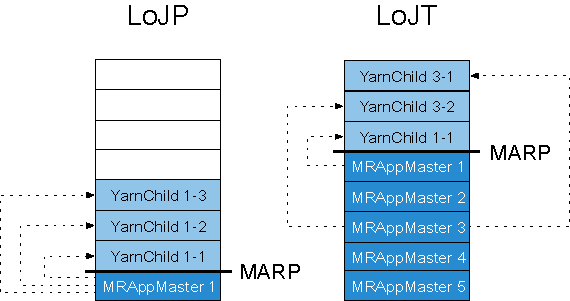
\includegraphics{./images/marpValue.pdf}
    \caption[LoJP und LoJT in Hadoop]
    {LoJP und LoJT in Hadoop (entnommen aus \cite{zhang2016}).
    Während beim LoJP sehr viel Speicher für Anwendungscontainer ungenutzt bleibt, können beim LoJT nicht genügend Anwendungscontainer allokiert werden, um die Anwendungen auszuführen.}
    \label{fig:marpValue}
\end{figure}

Die Selfbalancing"=Komponente passt daher den \ac{MARP}"=Wert abhängig von der Speicherauslastung dynamisch zur Laufzeit an.
So wird der \ac{MARP}"=Wert verringert, wenn die Speicherauslastung sehr hoch ist, und erhöht, wenn die Speicherauslastung sehr niedrig ist \cite{zhang2016}.
Dadurch wird es ermöglicht, dass die maximal mögliche Anzahl an Anwendungen ausgeführt werden kann.
Die Evaluation von \citeauthor{zhang2016} ergab zudem, dass die dynamische Anpassung des \ac{MARP}"=Wertes darüber hinaus auch effizienter ist als eine manuelle, statische Optimierung.

\subsection{Analyse der Selfbalancing"=Komponente}
\label{sec:selfbalancingAnalysis}

Da in dieser Fallstudie auch Mutationstests zum Einsatz kommen, bei denen die Selfbalancing"=Komponente entsprechend verändert wird (vgl. \autoref{sec:implMutationTests}), wurde die Komponente zunächst analyisiert.
Sie besteht aus folgenden vier Java"=Klassen, welche den Kern der Komponente darstellen, und drei Shell"=Scripten, die als Verbindung zum Hadoop"=Cluster dienen:

\begin{itemize}
    \item Java"=Klassen:
    \begin{itemize}
        \item \texttt{controller.Controller}
        \item \texttt{effectuator.Effectuator}
        \item \texttt{monitor.ControlNodeMonitor}
        \item \texttt{monitor.MemUtilization}
    \end{itemize}
    \item Shell"=Scripte:
    \begin{itemize}
        \item \texttt{selfTuning-CapacityScheduler.sh}
        \item \texttt{selfTuning-controlNode.sh}
        \item \texttt{selfTuning-mem-controlNode.sh}
    \end{itemize}
\end{itemize}

Um den Zustand von Hadoop korrekt zu ermitteln, wird ein Kalman"=Filter in Form der Open"=Source"=Bibliotek JKalman\footnote{\url{https://jkalman.sourceforge.io/}} genutzt.
Der Kalman"=Filter wurde von \citeauthor{Kalman1960} erstmals in \cite{Kalman1960} beschrieben und dient, um \enquote{aus verrauschten und teils redundanten Messungen die Zustände und Parameter des Systems zu schätzen} und lässt sich aufgrund seines Aufbaus auch für Echtzeitanwendungen nutzen \cite{Marchthaler2017}.
Als einfaches Anwendungsbeispiel hierfür ist in \cite{Marchthaler2017} die Apollo"=Mondlandefähre genannt, \citeauthor{Strukov2001} nutzte ihn in \cite{Strukov2001} aber auch zur Reduktion der Komplexität im Controlling.
Für weitere Informationen zum Kalman"=Filter wie seinen Aufbau, Funktionsweise und Anwendung sei hier auf entsprechende Fachliteratur wie \zB \cite{Kim2016,Simon2006,Aggoun2004} verwiesen.

Die drei Shell-Scripte dienen zur Interaktion zwischen dem Controller der Selfbalancing"=Komponente und Hadoop selbst.
Die beiden zuletzt genannten Scripte werden von den beiden Monitor"=Klassen sekündlich gestartet und ermitteln basierend auf den Logs die Auslastung des Clusters.
Mithilfe von \texttt{selfTuning-controlNode.sh}, das von \texttt{ControlNodeMonitor} gestartet wird, wird die Anzahl an aktiven und wartenden YARN"=Jobs ermittelt und anschließend in die \texttt{controlNodeLog}"=Datei geschrieben.
Durch die Ausführung von \texttt{selfTuning-mem-controlNode.sh} (gestartet durch \texttt{MemUtilization}) wird dagegen die Auslastung des Arbeitsspeichers ermittelt und in die \texttt{memLog}"=Datei geschrieben.

Die in den beiden Dateien enthaltenen Werten im Anschluss wiederum sekündlich vom \texttt{Controller} ausgelesen und mithilfe des Kalman"=Filters bereinigt.
Anschließend werden die bereits in \cite{zhang2016} vorgestellten Algorithmen zum Ermitteln des neuen \ac{MARP}"=Wertes ausgeführt, damit dieser entsprechend erhöht bzw. verringert wird.

Um den dadurch neu ermittelten \ac{MARP}"=Wert anzuwenden, wird abschließend mithilfe des \texttt{Effectuator}s das dritte Shell"=Script \texttt{selfTuning-CapacityScheduler.sh} ausgeführt.
Mithilfe dieses Shell"=Scriptes wird der neue MARP"=Wert in der Konfiguration des \emph{Capacity Schedulers} gespeichert.
